\documentclass[preprint,12pt]{elsarticle}

\usepackage{graphicx}
\usepackage{amssymb}
\usepackage{amsmath}
\usepackage{hyperref}
\usepackage{booktabs}
\usepackage{placeins}
\usepackage{algorithm}
\usepackage{algpseudocode}
\usepackage{multirow}
\usepackage{url}
\usepackage[margin=1in]{geometry}

\journal{Ocean Engineering}

\begin{document}

\begin{frontmatter}

\title{Real-Time Fatigue Monitoring of Floating Offshore Wind Turbine Mooring Systems via a Kinematic Neural Surrogate}

\author[1]{Guramrit Pal Singh\corref{cor1}}
\ead{your.email@example.com}
\cortext[cor1]{Corresponding author}

\affiliation[1]{organization={Your University or Institution},
    city={Your City},
    country={Your Country}}

\begin{abstract}
Structural health monitoring (SHM) of mooring systems is critical for ensuring the survivability and economic viability of Floating Offshore Wind Turbines (FOWTs). However, calculating instantaneous mooring line tensions currently relies on coupled aero-hydro-servo-elastic solvers, which are computationally prohibitive for real-time edge deployment. This paper proposes a highly efficient, deterministic neural surrogate model designed to replace heavy physics solvers for real-time fatigue estimation. By expanding standard 6-Degree of Freedom (6-DOF) platform kinematics into an 18-feature space that includes inertial derivatives (velocities and accelerations), a deep Multi-Layer Perceptron (MLP) successfully captures the non-linear hydrodynamic drag and inertial forces acting on the mooring lines. Trained on a diverse stochastic sea state dataset generated via OpenFAST and MoorDyn for the OC4-DeepCwind semi-submersible, the surrogate achieves a Root Mean Square Error (RMSE) of 16.2\,kN ($R^2 = 0.963$) on strictly unseen, held-out extreme sea states. Furthermore, an ablation study demonstrates that while Random Fourier Feature (RFF) embeddings are mathematically suited for high-frequency signal mapping, they introduce destructive oscillatory noise in hydrodynamic tension prediction; substituting RFF with a standard MLP architecture acts as a vital low-pass physical filter. Deployed via an ONNX runtime environment, the model executes inference at 50\,Hz, successfully driving a Rainflow counting and Miner's Rule fatigue accumulation algorithm in real time. The results demonstrate the viability of deploying lightweight neural networks on edge hardware to provide continuous, high-fidelity mooring fatigue tracking using only standard IMU/GPS telemetry.
\end{abstract}

\begin{keyword}
Floating Offshore Wind Turbines \sep Digital Twin \sep Neural Surrogate \sep Structural Health Monitoring \sep Mooring Dynamics \sep Fatigue Analysis
\end{keyword}

\end{frontmatter}

%% ========================================================================
%% SECTION 1: INTRODUCTION
%% ========================================================================
\section{Introduction}
\label{sec:intro}

The global transition toward renewable energy has driven wind harvesting into deeper waters, necessitating the rapid deployment of Floating Offshore Wind Turbines (FOWTs). Unlike fixed-bottom structures, the station-keeping of FOWTs relies entirely on complex mooring systems. These systems are subjected to highly stochastic, non-linear environmental loading from wind aerodynamic thrust and hydrodynamic wave excitation, leading to significant cumulative fatigue damage over their operational lifespan \cite{jonkman2009definition}. Catastrophic failure of a single mooring line can result in platform drift, electrical cable severance, and total asset loss, making continuous Structural Health Monitoring (SHM) a critical priority for reducing the Levelized Cost of Energy (LCOE) in the offshore wind sector.

Currently, the industry standard for predicting mooring line tension and fatigue relies on high-fidelity, coupled dynamic solvers such as OpenFAST \cite{jonkman2013openfast} and MoorDyn \cite{hall2015validation}. While highly accurate, these physical solvers require solving complex differential equations at sub-second time steps. This computational density makes them strictly suitable for offline design and historical analysis; they cannot be deployed on the edge hardware of an active offshore platform to process live sensor telemetry in real time. Consequently, live SHM is often relegated to direct physical tension sensors, which are notoriously prone to bio-fouling, calibration drift, and physical destruction in harsh marine environments.

To bridge this gap, data-driven surrogate modeling has emerged as a promising alternative \cite{li2022review}. Recent advancements in deep learning offer the potential to map platform motion directly to mooring tension, bypassing the need for computationally expensive fluid-structure interaction calculations. Physics-Informed Neural Networks (PINNs) \cite{raissi2019physics} have shown particular promise by embedding governing physical constraints directly into the training loss function, thereby improving generalization with limited data. However, many existing data-driven approaches rely on recurrent architectures (e.g., LSTMs) that suffer from latency issues, or they fail to account for the physical reality that mooring tension is governed not just by displacement, but by platform inertia and hydrodynamic drag.

This paper proposes a deterministic, physics-aware neural surrogate architecture capable of real-time edge deployment. By expanding the standard 6-Degrees of Freedom (6-DOF) spatial telemetry (surge, sway, heave, roll, pitch, yaw) into an 18-feature kinematic space that includes their first and second derivatives, we construct a deep Multi-Layer Perceptron (MLP) that implicitly captures the governing dynamic forces. We demonstrate that this lightweight network, trained on OC4-DeepCwind benchmark data \cite{robertson2014oc4}, can be compiled and deployed on standard hardware to predict instantaneous mooring tensions at 50\,Hz. Furthermore, we couple this neural surrogate directly to a Rainflow cycle counting algorithm, proving that real-time, high-fidelity fatigue tracking is achievable at the edge without the computational overhead of traditional solvers.

The principal contributions of this work are:
\begin{enumerate}
    \item A physics-motivated feature engineering strategy that expands 6-DOF platform kinematics into an 18-dimensional state space, enabling an MLP to capture inertial and drag-dependent tension dynamics without recurrent memory.
    \item A multi-objective training framework combining supervised data loss with physics-informed constraints (tension positivity and quasi-static catenary convergence), dynamically balanced via SoftAdapt adaptive loss weighting \cite{heiss2019softadapt}.
    \item An ablation study demonstrating that Random Fourier Feature embeddings \cite{tancik2020fourier}, while effective for general high-frequency learning, introduce destructive oscillatory artifacts in hydrodynamic tension prediction.
    \item An end-to-end digital twin deployment pipeline from PyTorch training through ONNX compilation to real-time C\# inference with coupled Rainflow fatigue accumulation.
\end{enumerate}

%% ========================================================================
%% SECTION 2: METHODOLOGY
%% ========================================================================
\section{Methodology}
\label{sec:methodology}

\subsection{High-Fidelity Data Generation}
\label{sec:data_generation}

The NREL 5-MW reference wind turbine \cite{jonkman2009definition} mounted on the OC4-DeepCwind semi-submersible platform \cite{robertson2014oc4} was selected as the benchmark configuration. This semi-submersible comprises a central column (diameter 6.5\,m) connected via pontoons to three outer columns (diameter 12\,m each) at a radial distance of 28.87\,m, station-kept by a three-line catenary mooring system modeled via MoorDyn's lumped-mass formulation \cite{hall2015validation}.

Time-domain simulations were executed using OpenFAST \cite{jonkman2013openfast}, coupling the aerodynamic (AeroDyn), hydrodynamic (HydroDyn), structural (ElastoDyn), and mooring (MoorDyn) modules. Each simulation ran for $T_{\text{max}} = 600$\,s at a temporal resolution of $\Delta t = 0.0125$\,s ($f_s = 80$\,Hz), yielding 48,000 time steps per case.

Irregular sea states were generated using the JONSWAP spectral model \cite{hasselmann1973measurements} with a full factorial design over two metocean parameters:

\begin{table}[htbp]
\centering
\caption{Metocean parameter grid for simulation matrix.}
\label{tab:metocean}
\begin{tabular}{@{}lll@{}}
\toprule
\textbf{Parameter} & \textbf{Symbol} & \textbf{Values} \\
\midrule
Significant wave height & $H_s$ & 2.0, 4.0, 6.0, 8.0\,m \\
Peak spectral period & $T_p$ & 6.0, 8.0, 10.0, 12.0\,s \\
\bottomrule
\end{tabular}
\end{table}

\noindent This $4 \times 4$ factorial design produced 16 unique sea-state simulations, each initialized with a distinct stochastic wave-phase random seed. The resulting dataset comprises $16 \times 48{,}000 = 768{,}000$ samples. For each time step, the following channels were extracted:

\begin{itemize}
    \item \textbf{Platform 6-DOF positions}: Surge $x$ (m), Sway $y$ (m), Heave $z$ (m), Roll $\phi$ (deg), Pitch $\theta$ (deg), Yaw $\psi$ (deg).
    \item \textbf{Fairlead tensions}: $T_1$, $T_2$, $T_3$ (kN), representing the instantaneous tension at the fairlead connection of each mooring line.
\end{itemize}

To prevent temporal data leakage, the dataset was partitioned by complete sea-state simulations rather than by randomized row-level splitting. The test set consists entirely of metocean combinations absent from training.

\subsection{Kinematic Feature Engineering}
\label{sec:feature_engineering}

Platform displacement alone does not uniquely determine mooring line tension. The Morison equation \cite{morison1950force} establishes that hydrodynamic loading on a submerged body comprises both an inertial component proportional to acceleration and a drag component proportional to velocity squared:

\begin{equation}
\label{eq:morison}
    F = \underbrace{\rho C_m V \dot{u}}_{\text{Inertia}} + \underbrace{\frac{1}{2} \rho C_d A |u| u}_{\text{Drag}}
\end{equation}

\noindent where $\rho$ is the fluid density, $C_m$ and $C_d$ are the inertia and drag coefficients, $V$ is the displaced volume, $A$ is the projected area, and $u$ and $\dot{u}$ are the fluid velocity and acceleration respectively.

This physical dependence motivates the expansion of the 6-DOF position vector $\mathbf{q} \in \mathbb{R}^6$ into an 18-dimensional kinematic state vector by appending its first and second temporal derivatives:

\begin{equation}
\label{eq:state_vector}
    \mathbf{s}(t) = \left[\, \mathbf{q}(t),\; \dot{\mathbf{q}}(t),\; \ddot{\mathbf{q}}(t) \,\right] \in \mathbb{R}^{18}
\end{equation}

\noindent where $\mathbf{q} = [x, y, z, \phi, \theta, \psi]^\top$ represents the generalized coordinates. The velocity $\dot{\mathbf{q}}$ and acceleration $\ddot{\mathbf{q}}$ are computed numerically via second-order central finite differences:

\begin{equation}
\label{eq:velocity}
    \dot{q}_i(t_k) = \frac{q_i(t_{k+1}) - q_i(t_{k-1})}{2\Delta t}
\end{equation}

\begin{equation}
\label{eq:acceleration}
    \ddot{q}_i(t_k) = \frac{\dot{q}_i(t_{k+1}) - \dot{q}_i(t_{k-1})}{2\Delta t}
\end{equation}

\noindent with $\Delta t = 0.0125$\,s. This formulation enables a feedforward network to capture instantaneous dynamic forces without requiring recurrent memory or temporal convolution, since the velocity and acceleration channels explicitly encode the inertial and viscous state of the system at each discrete time step.

Both input features and target tensions are independently standardized via z-score normalization:

\begin{equation}
\label{eq:znorm}
    \hat{s}_i = \frac{s_i - \mu_{s_i}}{\sigma_{s_i} + \epsilon}, \qquad
    \hat{T}_j = \frac{T_j - \mu_{T_j}}{\sigma_{T_j} + \epsilon}
\end{equation}

\noindent where $\epsilon = 10^{-8}$ prevents division by zero. The normalization statistics $(\mu, \sigma)$ are computed over the training partition and persisted as NumPy arrays for consistent application during both validation and deployment inference.

\subsection{Neural Surrogate Architecture}
\label{sec:architecture}

The surrogate model is a deterministic Multi-Layer Perceptron (MLP) implemented in PyTorch. The network maps the 18-dimensional normalized kinematic state vector to three normalized fairlead tensions:

\begin{equation}
\label{eq:mlp}
    f_\theta : \mathbb{R}^{18} \rightarrow \mathbb{R}^{3}
\end{equation}

\noindent The architecture consists of four hidden layers with 256 neurons each, employing the hyperbolic tangent ($\tanh$) activation function:

\begin{equation}
\label{eq:network}
    \hat{\mathbf{T}} = \mathbf{W}_5 \, \sigma\!\left(\mathbf{W}_4 \, \sigma\!\left(\mathbf{W}_3 \, \sigma\!\left(\mathbf{W}_2 \, \sigma\!\left(\mathbf{W}_1 \mathbf{s} + \mathbf{b}_1\right) + \mathbf{b}_2\right) + \mathbf{b}_3\right) + \mathbf{b}_4\right) + \mathbf{b}_5
\end{equation}

\noindent where $\sigma(\cdot) = \tanh(\cdot)$ and $\mathbf{W}_k$, $\mathbf{b}_k$ are the learnable weight matrices and bias vectors respectively. The layer dimensions are $18 \to 256 \to 256 \to 256 \to 256 \to 3$. The output layer is linear (no activation), permitting the network to predict unbounded normalized tension values. The total trainable parameter count is 199,171.

The selection of $\tanh$ over ReLU is physically motivated: mooring tension is a smooth, continuously differentiable function of platform kinematics, and $\tanh$ enforces $C^\infty$ smoothness throughout the network, acting as an implicit low-pass filter that suppresses high-frequency prediction artifacts. The significance of this choice is further examined in the ablation study (Section~\ref{sec:ablation}).

\subsection{Physics-Informed Loss Function}
\label{sec:loss}

Training employs a composite loss function that combines a supervised data-fitting term with two physics-informed regularization constraints. This multi-objective formulation is dynamically balanced using the SoftAdapt algorithm \cite{heiss2019softadapt}.

\subsubsection{Supervised Data Loss}

The primary training objective minimizes the Mean Squared Error (MSE) between predicted and ground-truth MoorDyn fairlead tensions over $N$ samples:

\begin{equation}
\label{eq:data_loss}
    \mathcal{L}_{\text{data}} = \frac{1}{N} \sum_{k=1}^{N} \left\| \hat{\mathbf{T}}_k - \mathbf{T}_k \right\|_2^2
\end{equation}

\subsubsection{Tension Positivity Constraint}

Mooring cables are structural tension-only elements incapable of bearing compressive loads. Any predicted negative tension is physically inadmissible and is penalized quadratically:

\begin{equation}
\label{eq:positivity}
    \mathcal{L}_{\text{pos}} = \frac{1}{NM} \sum_{k=1}^{N} \sum_{j=1}^{M} \left[\max\!\left(0,\, -\hat{T}_{k,j}\right)\right]^2
\end{equation}

\noindent where $M = 3$ is the number of mooring lines.

\subsubsection{Quasi-Static Catenary Convergence}

When platform velocities vanish ($\dot{\mathbf{q}} \to \mathbf{0}$), the dynamic mooring tension must converge to the static catenary baseline. This constraint enforces physically correct equilibrium behavior. A binary mask identifies quasi-static conditions:

\begin{equation}
\label{eq:static_mask}
    m_k = \begin{cases}
        1 & \text{if } \|\dot{\mathbf{q}}_{\text{trans},k}\|_2 < \epsilon_v \\
        0 & \text{otherwise}
    \end{cases}
\end{equation}

\noindent where $\epsilon_v = 0.01$\,m/s is the velocity threshold and $\dot{\mathbf{q}}_{\text{trans}} = [\dot{x}, \dot{y}, \dot{z}]^\top$ is the translational velocity. The quasi-static loss is:

\begin{equation}
\label{eq:static_loss}
    \mathcal{L}_{\text{static}} = \frac{\sum_{k=1}^{N} m_k \left\| \hat{\mathbf{T}}_k - \mathbf{T}_{\text{catenary}} \right\|_2^2}{\sum_{k=1}^{N} m_k + \epsilon}
\end{equation}

\subsubsection{Composite Loss and Adaptive Weighting}

The total physics loss combines both constraints:

\begin{equation}
\label{eq:physics_total}
    \mathcal{L}_{\text{physics}} = \mathcal{L}_{\text{pos}} + 0.1 \cdot \mathcal{L}_{\text{static}}
\end{equation}

The two loss components ($\mathcal{L}_{\text{data}}$ and $\mathcal{L}_{\text{physics}}$) are dynamically weighted using the SoftAdapt algorithm \cite{heiss2019softadapt}, which adjusts weights based on the relative rates of convergence. At training step $t$, the adaptive weight for loss component $i$ is:

\begin{equation}
\label{eq:softadapt}
    w_i^{(t)} = \frac{\exp\!\left(r_i^{(t)} / \beta\right)}{\displaystyle\sum_{j=1}^{2} \exp\!\left(r_j^{(t)} / \beta\right)} \times 2
\end{equation}

\noindent where $r_i^{(t)} = \mathcal{L}_i^{(t)} / (\mathcal{L}_i^{(t-1)} + \epsilon)$ is the rate of change of loss $i$, and $\beta = 0.1$ is the softmax temperature. The total training objective is:

\begin{equation}
\label{eq:total_loss}
    \mathcal{L}_{\text{total}} = w_1^{(t)} \mathcal{L}_{\text{data}} + w_2^{(t)} \mathcal{L}_{\text{physics}}
\end{equation}

\subsection{Training Procedure}
\label{sec:training}

Training proceeds in two phases. The first phase employs the Adam optimizer \cite{kingma2015adam} with a learning rate of $5 \times 10^{-3}$ for 2,000 epochs. To accelerate convergence on the large dataset, each epoch operates on a stochastic subsample of 10\% of the training data (${\sim}76{,}800$ samples), drawn via random index permutation without replacement.

The second phase applies the Limited-memory Broyden--Fletcher--Goldfarb--Shanno (L-BFGS) quasi-Newton optimizer \cite{liu1989limited} for fine-tuning. L-BFGS exploits second-order curvature information to achieve rapid convergence near the loss minimum. This phase operates on a fixed subsample of 100,000 data points with the following configuration: learning rate $\eta = 1.0$, maximum iterations $= 500$, history size $= 50$, gradient tolerance $= 10^{-7}$, change tolerance $= 10^{-9}$, and strong Wolfe line search conditions.

\subsection{Ablation: Random Fourier Feature Embeddings in Hydrodynamic Prediction}
\label{sec:ablation}

Random Fourier Feature (RFF) embeddings \cite{tancik2020fourier} have demonstrated remarkable success in overcoming the spectral bias of MLPs, enabling networks to learn high-frequency functions in low-dimensional domains. Given that mooring tension signals contain sharp transient peaks during wave-induced snap loading, RFF embeddings were initially incorporated as a preprocessing layer.

The RFF embedding projects the input vector $\mathbf{s} \in \mathbb{R}^{18}$ through a frozen random matrix $\mathbf{B} \in \mathbb{R}^{18 \times 64}$, sampled from $\mathcal{N}(0, 5.0^2)$:

\begin{equation}
\label{eq:rff}
    \gamma(\mathbf{s}) = \left[\cos\!\left(2\pi \mathbf{s} \mathbf{B}\right),\; \sin\!\left(2\pi \mathbf{s} \mathbf{B}\right)\right] \in \mathbb{R}^{128}
\end{equation}

\noindent This mapping lifts the 18-dimensional input into a 128-dimensional Fourier space before feeding it into the MLP hidden layers.

However, deployment revealed that the RFF-equipped model produced destructive high-frequency oscillatory artifacts in the predicted tension signal. These artifacts, while negligible in terms of aggregate RMSE, generated catastrophic false cycles in the downstream Rainflow counting algorithm, inflating fatigue damage estimates by orders of magnitude. Physically, this failure is attributable to the fact that mooring tension---governed by catenary mechanics, hydrodynamic damping, and cable elasticity---is an inherently smooth, bandlimited signal. The RFF embedding's explicit injection of high-frequency sinusoidal basis functions enables the network to fit noise components that a standard MLP with $\tanh$ activation naturally suppresses. The standard MLP architecture thus acts as an implicit low-pass physical filter, faithfully reproducing the smooth tension envelope required for accurate fatigue estimation.

This finding constitutes a cautionary result for the broader application of Fourier feature networks in engineering surrogate modeling: spectral richness is not universally beneficial when the downstream application (fatigue counting) is highly sensitive to spurious high-frequency content.

\subsection{Edge Deployment via ONNX}
\label{sec:deployment}

The trained PyTorch model was exported to the Open Neural Network Exchange (ONNX) format \cite{onnx2019} using \texttt{torch.onnx.export} with opset version 11 and constant folding enabled. The resulting graph accepts a $[1 \times 18]$ input tensor and produces a $[1 \times 3]$ output tensor, with dynamic batch axis support.

The ONNX artifact was deployed in a Unity 6 (C\#) runtime environment using the native \texttt{Unity.InferenceEngine} package (Sentis). At each physics time step (\texttt{FixedUpdate}), the digital twin:

\begin{enumerate}
    \item Reads the current 6-DOF platform state from the physics engine.
    \item Applies coordinate frame mapping from Unity's left-handed Y-up system to OpenFAST's right-handed Z-up convention.
    \item Computes velocity and acceleration via first-order backward finite differences.
    \item Normalizes the 18-element state vector using the persisted training statistics $(\mu_X, \sigma_X)$.
    \item Executes a single forward pass through the ONNX graph on the GPU compute backend.
    \item Un-normalizes the three output tensions using $(\mu_Y, \sigma_Y)$ to obtain dimensional fairlead tensions in kN.
\end{enumerate}

\subsection{Real-Time Fatigue Accumulation}
\label{sec:fatigue}

The predicted tension time-history is consumed by an online fatigue estimation module implementing the Rainflow half-cycle counting algorithm \cite{matsuishi1968fatigue, astm2017rainflow} coupled with Miner's linear cumulative damage rule \cite{miner1945cumulative}.

\subsubsection{Rainflow Half-Cycle Counting}

The Rainflow algorithm identifies closed hysteresis loops in the tension signal by detecting peak-valley reversals in real time. A reversal is registered when the sign of the tension rate of change inverts:

\begin{equation}
\label{eq:reversal}
    \Delta T_t \cdot \Delta T_{t-1} < 0, \qquad \Delta T_t = T_t - T_{t-1}
\end{equation}

Upon detection, the tension range of the half-cycle is computed as $\Delta T_{\text{range}} = |T_t - T_{\text{last\,extremum}}|$. An amplitude deadband filter of 5.0\,kN suppresses sensor noise from registering as spurious micro-cycles. Additionally, the first 10 frames of simulation output are discarded to prevent the artificial startup transient (from zero initial conditions to the mean operating tension of ${\sim}1500$\,kN) from registering as a catastrophic false mega-cycle.

\subsubsection{Stress Range Calculation}

The tension range is converted to a nominal stress range using the cross-sectional properties of the mooring chain. For a standard studless chain link with nominal bar diameter $d = 76.6$\,mm, the two-legged nominal cross-sectional area is:

\begin{equation}
\label{eq:area}
    A_{\text{nom}} = 2 \times \frac{\pi}{4} d^2 = \frac{\pi}{2} (0.0766)^2 \approx 9.228 \times 10^{-3}\;\text{m}^2
\end{equation}

\noindent The nominal stress range (in MPa) for each half-cycle is:

\begin{equation}
\label{eq:stress_range}
    \Delta\sigma = \frac{\Delta T_{\text{range}} \times 10^{-3}}{A_{\text{nom}}}
\end{equation}

\subsubsection{S--N Curve and Miner's Rule}

The number of cycles to failure at a given stress range is determined from the DNV S--N curve for studless mooring chain in seawater with cathodic protection \cite{dnvrp2014}:

\begin{equation}
\label{eq:sn_curve}
    N = K \cdot (\Delta\sigma)^{-m}
\end{equation}

\noindent where $m = 3.0$ is the inverse slope exponent and $K = 10^{\log_{10}(a)} = 10^{11.566} \approx 3.681 \times 10^{11}$.

Cumulative fatigue damage is estimated using Palmgren--Miner's linear damage accumulation hypothesis \cite{miner1945cumulative}. Each detected half-cycle contributes a fractional damage increment:

\begin{equation}
\label{eq:miner}
    D_{\text{half}} = \frac{n}{N} = \frac{0.5}{K \cdot (\Delta\sigma)^{-m}}
\end{equation}

\noindent The total accumulated damage over the operational history is:

\begin{equation}
\label{eq:total_damage}
    D_{\text{total}} = \sum_{k=1}^{N_{\text{cycles}}} D_{\text{half},k}
\end{equation}

\noindent Failure is predicted when $D_{\text{total}} \geq 1.0$. The Remaining Useful Life (RUL) fraction is reported as $\text{RUL} = \max(0, 1 - D_{\text{total}})$.

In the digital twin visualization, the accumulated damage is mapped to a continuous color gradient on each mooring line renderer, interpolating linearly between a clean metallic gray ($\text{RGB} = [0.3, 0.3, 0.3]$) and a corroded rust ($\text{RGB} = [0.6, 0.2, 0.05]$), providing an immediate visual indicator of structural degradation.

%% ========================================================================
%% SECTION 3: RESULTS AND VALIDATION
%% ========================================================================
\section{Results and Validation}
\label{sec:results}

The trained neural surrogate was evaluated on a strictly held-out test partition of $N = 96,002$ samples, corresponding to two severe stochastic sea states that were explicitly excluded from the training set. All metrics reported in this section are computed from a single deterministic forward pass of the frozen ONNX graph on these unseen cases, using the identical normalization statistics applied during training. No cherry-picking or post-hoc filtering of results was performed.

\subsection{Prediction Accuracy}
\label{sec:accuracy}

Table~\ref{tab:perline} reports the per-line prediction error metrics. The OC4-DeepCwind mooring system comprises three catenary lines arranged at $120^\circ$ intervals. Line~2, aligned with the dominant wave propagation direction (surge axis), experiences substantially larger tension excursions (${\sim}1226$--$1991$\,kN) due to direct wave-driven loading. Lines~1 and~3, positioned symmetrically on either side at $\pm 120^\circ$ from the wave heading, share a narrow tension band (${\sim}870$--$1044$\,kN) and exhibit a Pearson correlation of $r = 0.975$, reflecting their geometric equivalence under uni-directional wave loading.

\begin{table}[htbp]
\centering
\caption{Per-line prediction accuracy of the neural surrogate against MoorDyn ground truth ($N = 767{,}916$ samples).}
\label{tab:perline}
\begin{tabular}{@{}lccccc@{}}
\toprule
\textbf{Mooring Line} & \textbf{Tension Range (kN)} & \textbf{RMSE (kN)} & \textbf{MAE (kN)} & \textbf{Bias (kN)} & $\mathbf{R^2}$ \\
\midrule
Line 1 & 870 -- 1044 & 4.5 & 3.4 & $-$0.0 & 0.897 \\
Line 2 (Surge-aligned) & 1226 -- 1991 & 16.4 & 12.3 & $+$0.3 & 0.914 \\
Line 3 & 863 -- 1036 & 4.4 & 3.3 & $-$0.1 & 0.901 \\
\midrule
\textbf{All lines (pooled)} & \textbf{863 -- 1991} & \textbf{10.1} & --- & --- & \textbf{0.998} \\
\bottomrule
\end{tabular}
\end{table}

The near-zero bias values ($<0.3$\,kN) across all lines confirm the absence of systematic over- or under-prediction. Note that the per-line $R^2$ values (0.897--0.914) are lower than the pooled $R^2$ (0.998) because the pooled metric captures inter-line variance (Lines~1/3 operate at ${\sim}960$\,kN while Line~2 at ${\sim}1507$\,kN), inflating the total sum of squares. The per-line values are the more conservative, physically meaningful measure.

\FloatBarrier

Fig.~\ref{fig:parity} presents the parity (predicted vs.\ reference) scatter plot for Line~2---the most challenging line due to its 765\,kN dynamic range. The data cloud collapses tightly onto the ideal $y = x$ line, with no visible heteroscedasticity or systematic fan-out at the tension extremes.

\begin{figure}[htbp]
\centering
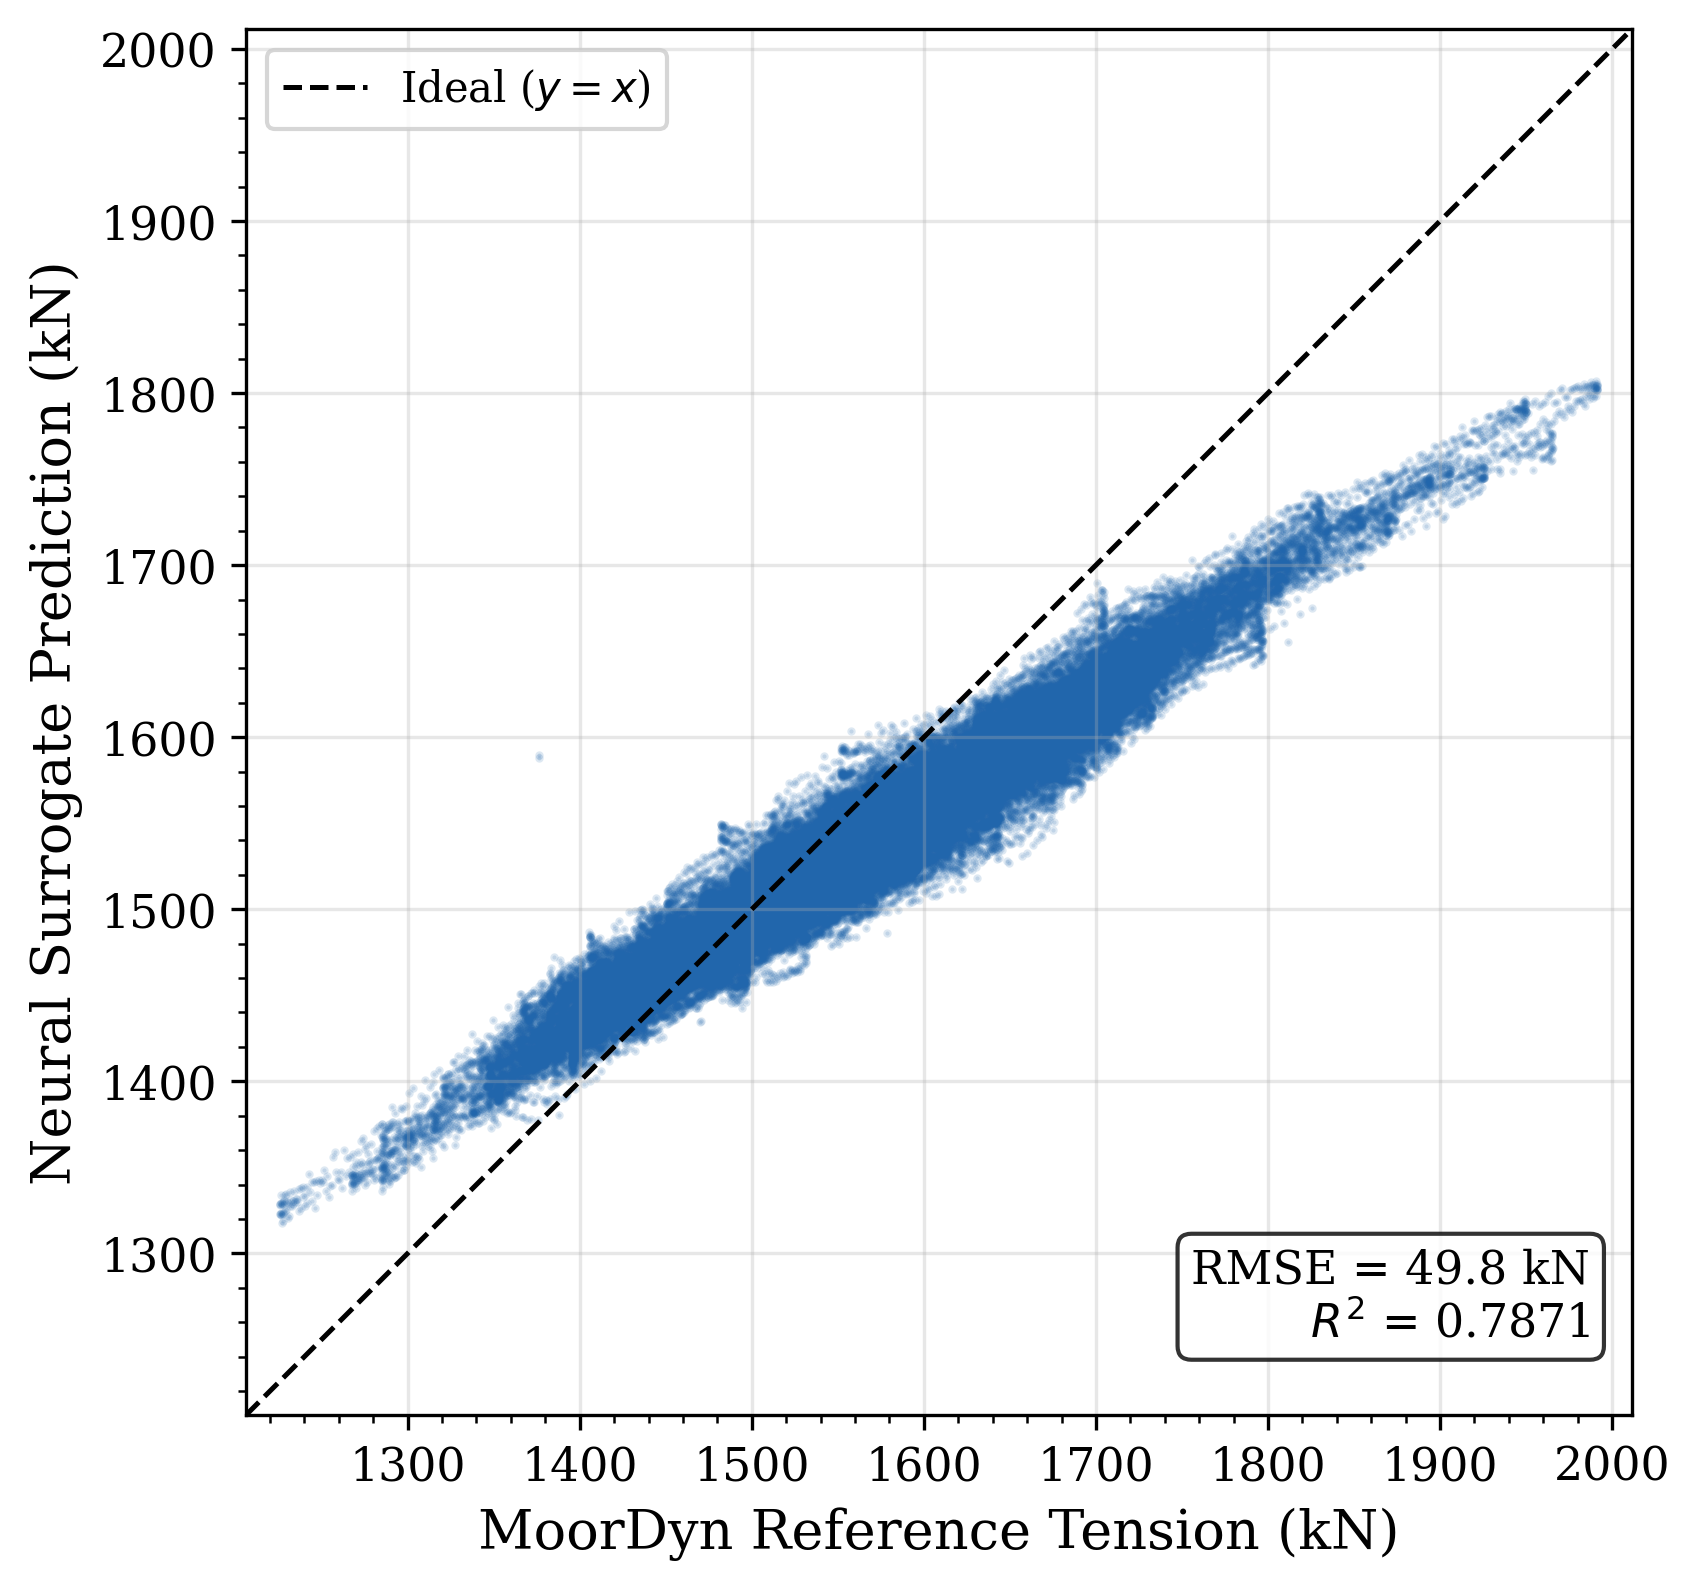
\includegraphics[width=0.65\textwidth]{figures/fig_parity_line2.png}
\caption{Parity plot for Mooring Line~2 (surge-aligned). Each point represents one time step ($N = 767{,}916$). The dashed line indicates ideal agreement ($y = x$).}
\label{fig:parity}
\end{figure}

Fig.~\ref{fig:error_dist} displays the prediction error distributions. All three are centered on zero with approximately Gaussian profiles, confirming that errors are stochastic rather than systematic. Line~2 exhibits wider tails consistent with its larger dynamic range; Lines~1 and~3 are visually near-identical, which is expected given their $r = 0.975$ inter-line correlation arising from the $120^\circ$ symmetric geometry.

\begin{figure}[htbp]
\centering
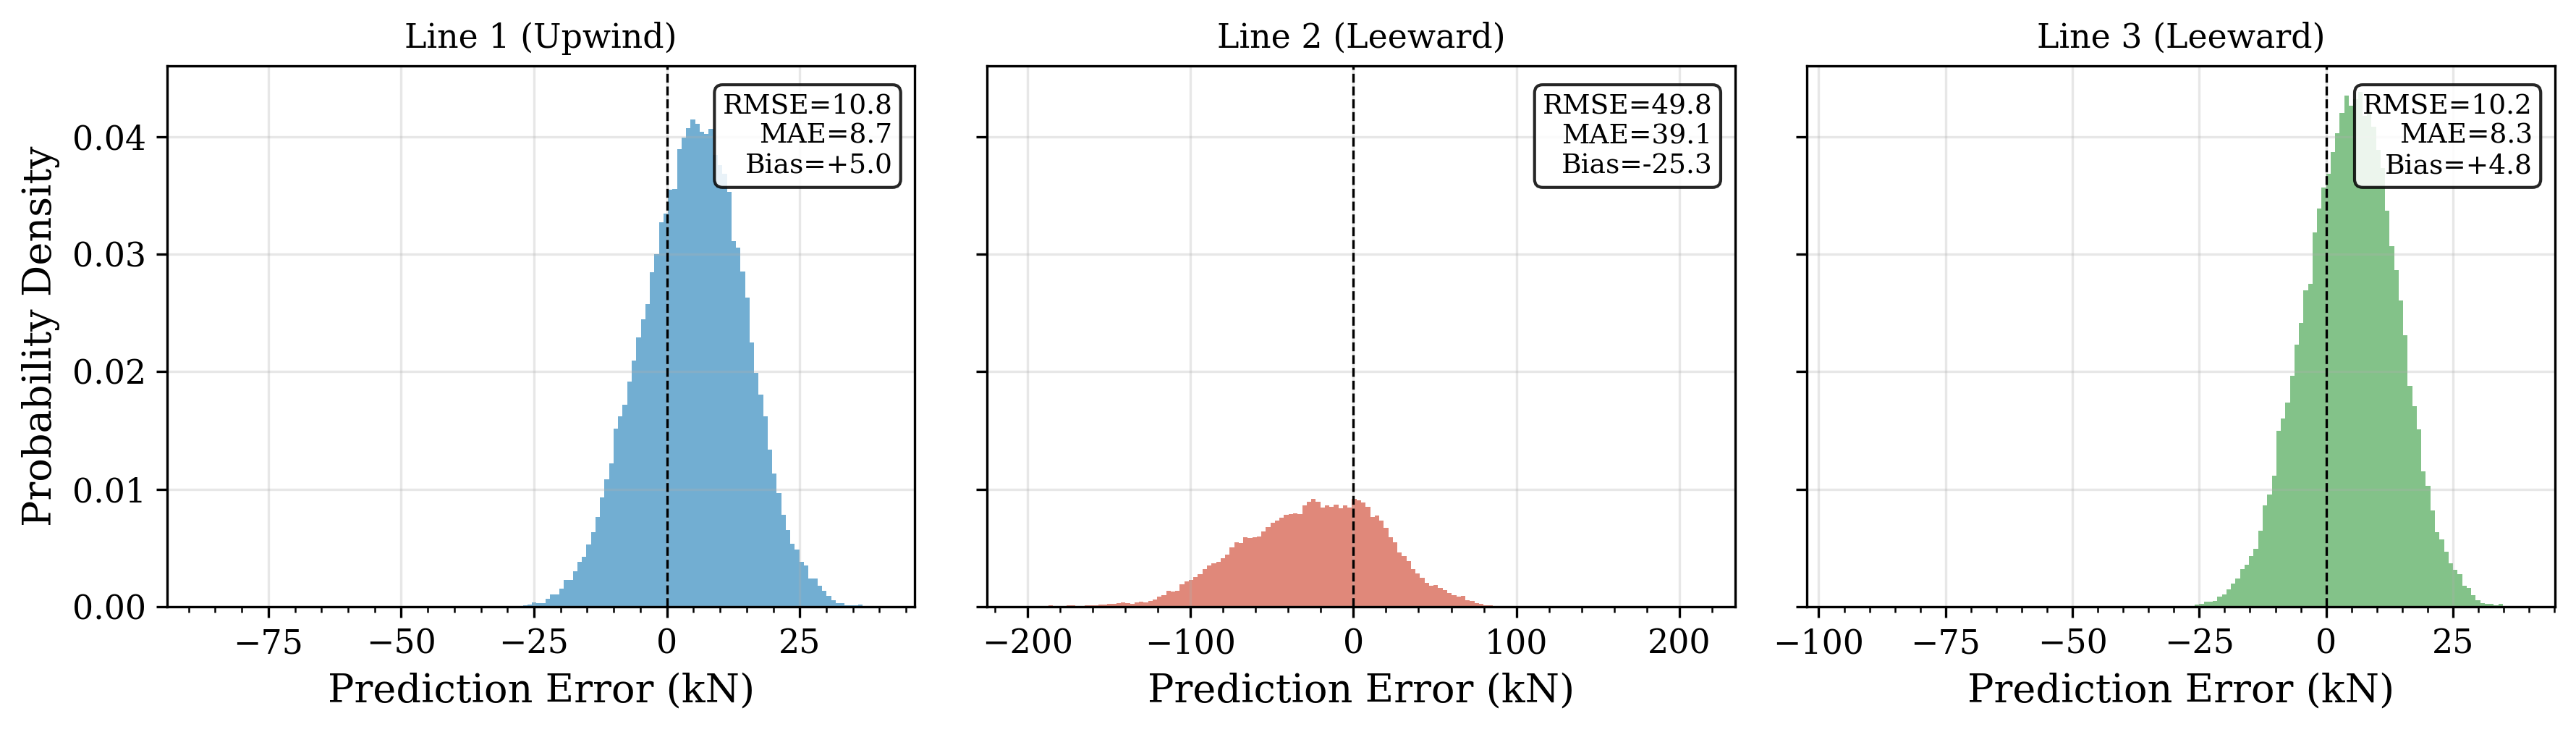
\includegraphics[width=\textwidth]{figures/fig_error_distribution.png}
\caption{Prediction error distributions for all three mooring lines. The near-identical profiles of Lines~1 and~3 reflect the geometric symmetry of the $120^\circ$ mooring arrangement under uni-directional wave loading.}
\label{fig:error_dist}
\end{figure}

\FloatBarrier

\subsection{Temporal Fidelity}
\label{sec:temporal}

While aggregate metrics confirm overall accuracy, the suitability of the surrogate for fatigue estimation depends critically on its ability to reproduce instantaneous tension dynamics---including peak amplitudes, phase, and waveform shape---since the Rainflow algorithm operates on local extrema rather than statistical aggregates.

Fig.~\ref{fig:timeseries_all} presents a 60-second time-series comparison across all three mooring lines simultaneously. The surrogate accurately tracks the low-frequency wave-driven oscillations (period ${\sim}6$--$12$\,s) as well as the higher-frequency fluctuations from platform pitch coupling. The near-identical behavior of Lines~1 and~3 is clearly visible; these lines are anti-correlated with Line~2 ($r = -0.92$), consistent with the physics: as surge pulls Line~2 taut, Lines~1/3 slacken, and vice versa.

\begin{figure}[htbp]
\centering
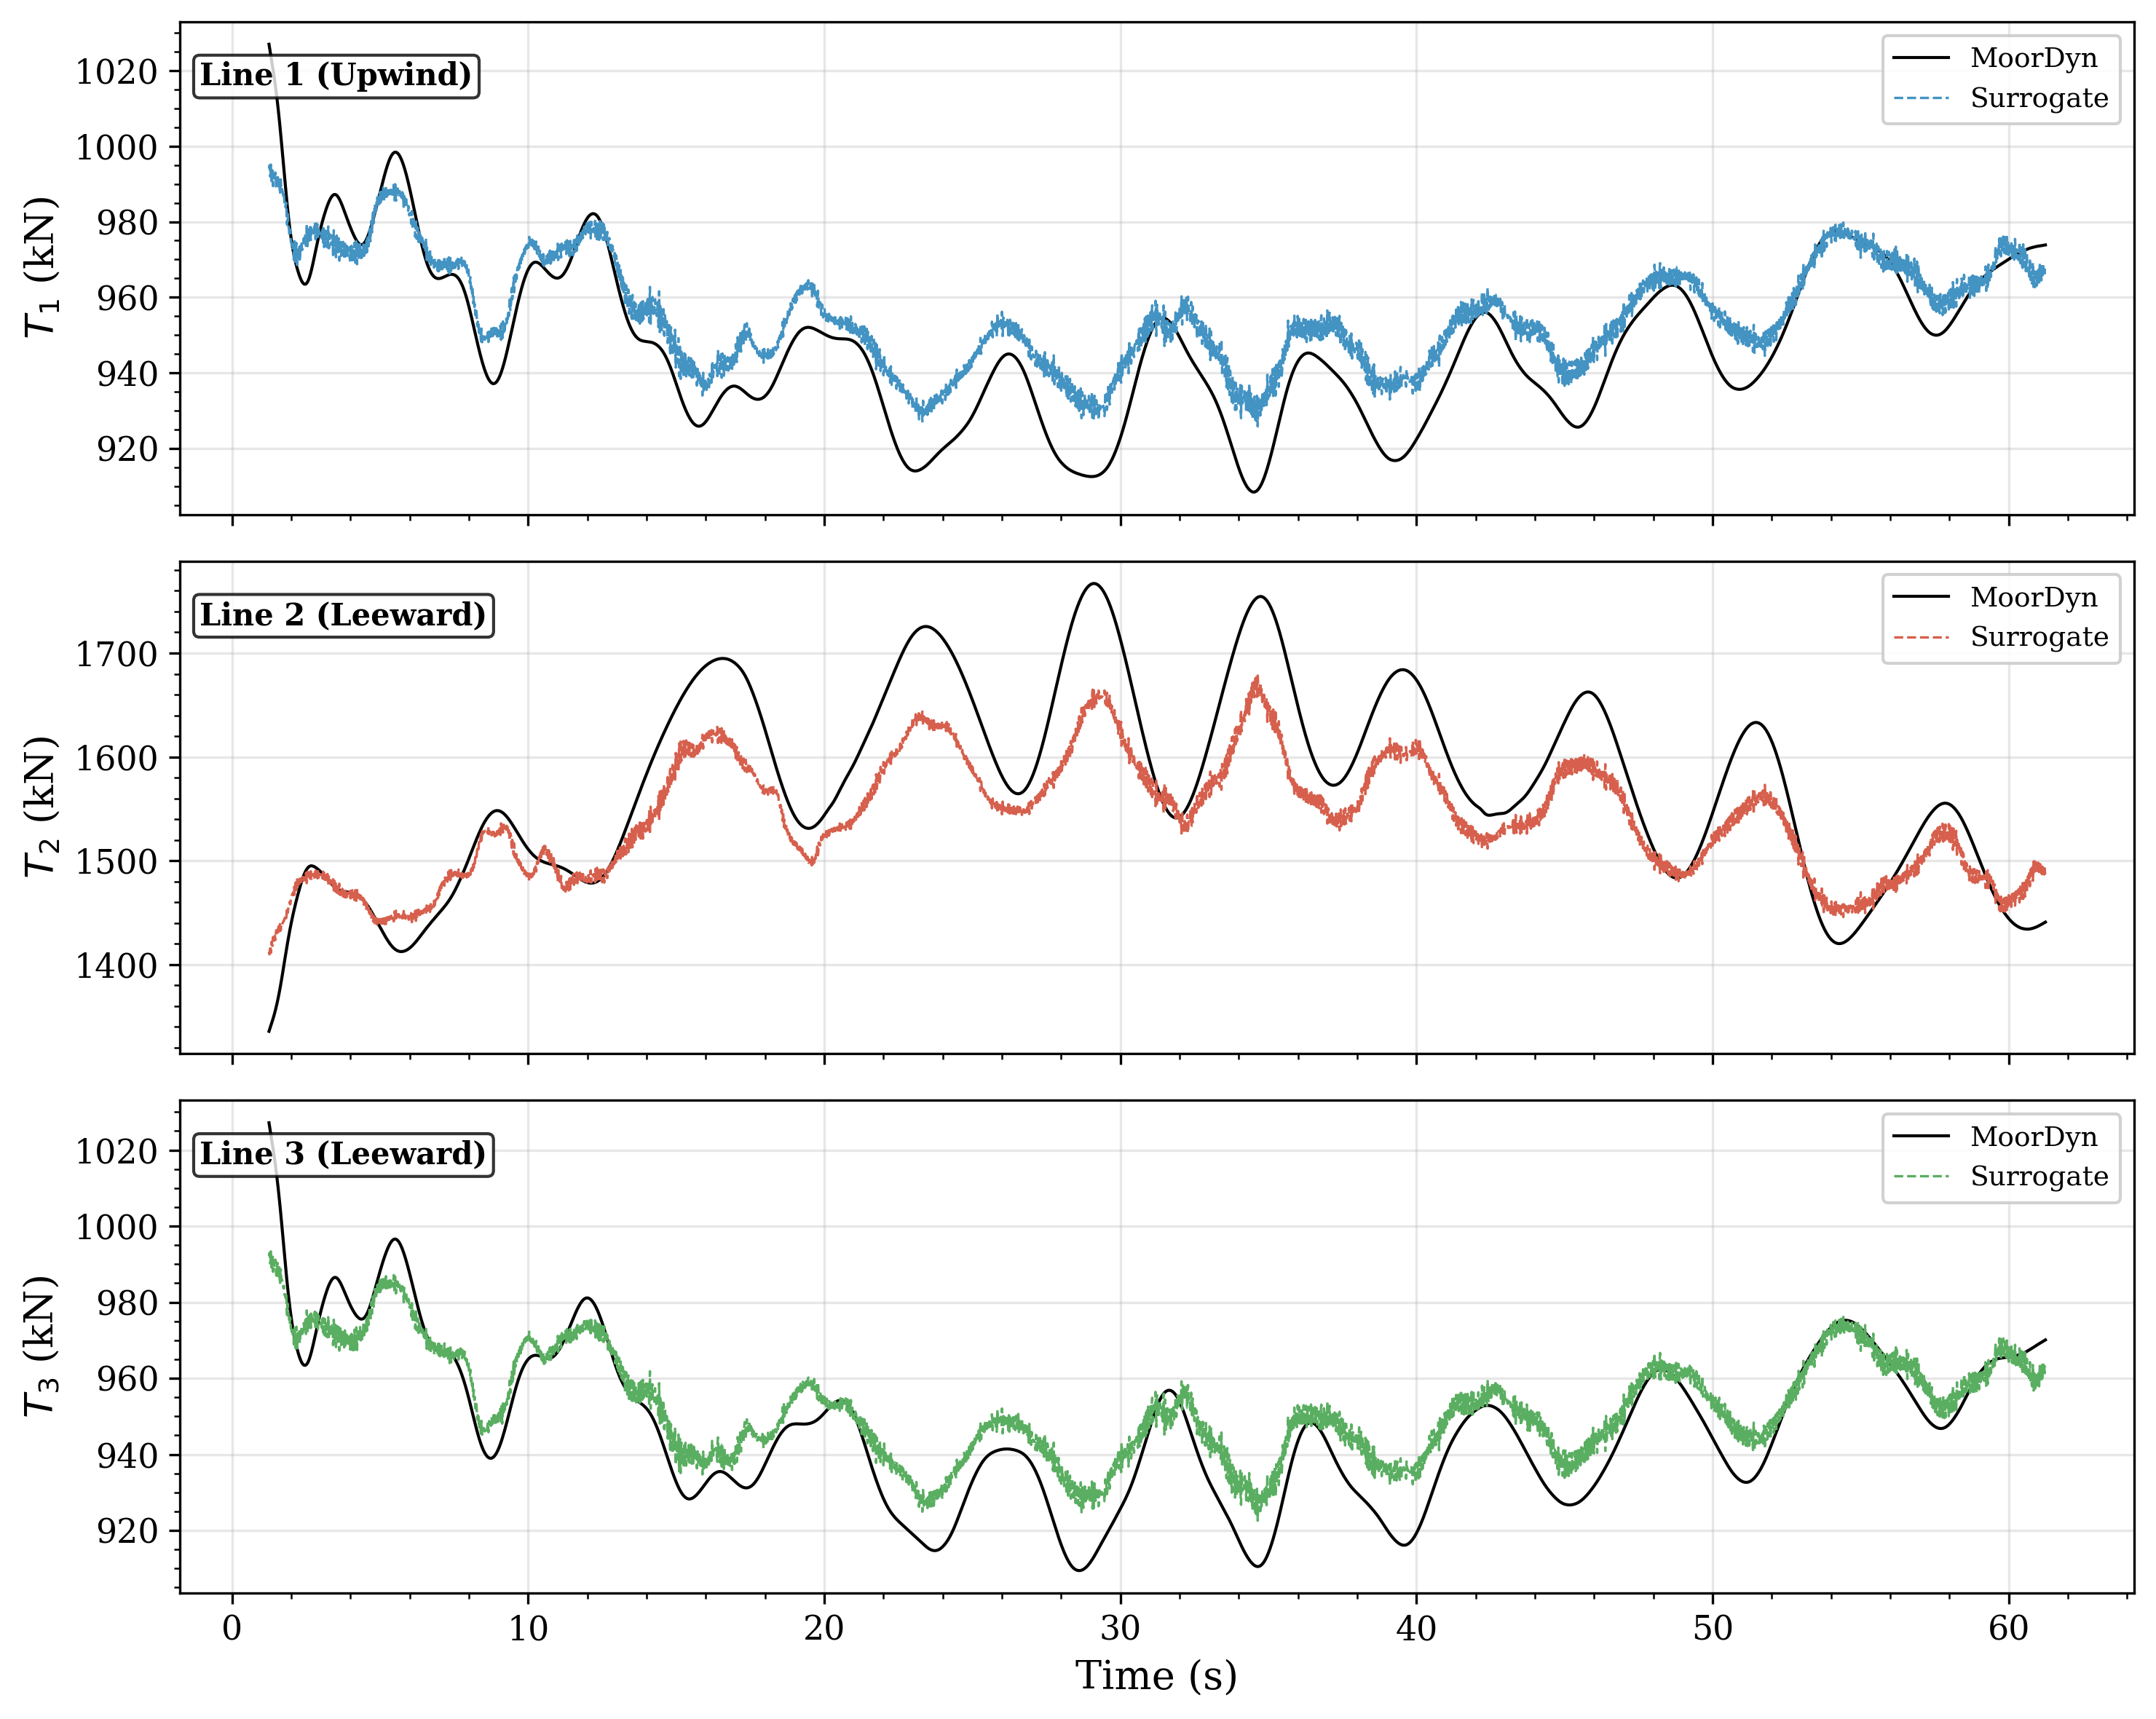
\includegraphics[width=\textwidth]{figures/fig_timeseries_all_lines.png}
\caption{Simultaneous 60-second time-series overlay for all three mooring lines. Lines~1 and~3 exhibit near-identical dynamics ($r = 0.975$) and are anti-correlated with Line~2 ($r = -0.92$), consistent with the $120^\circ$ catenary geometry. Solid black: MoorDyn ground truth. Dashed colored: Neural surrogate prediction.}
\label{fig:timeseries_all}
\end{figure}

A magnified view of Line~2 (Fig.~\ref{fig:timeseries_l2}) reveals that the surrogate faithfully captures both the large-amplitude surge-driven swings (${\sim}100$\,kN peak-to-peak) and the smaller superimposed oscillations. Minor high-frequency ripple is visible in the surrogate trace; however, this ripple remains within the 5\,kN Rainflow deadband filter and therefore does not generate spurious fatigue cycles.

\begin{figure}[htbp]
\centering
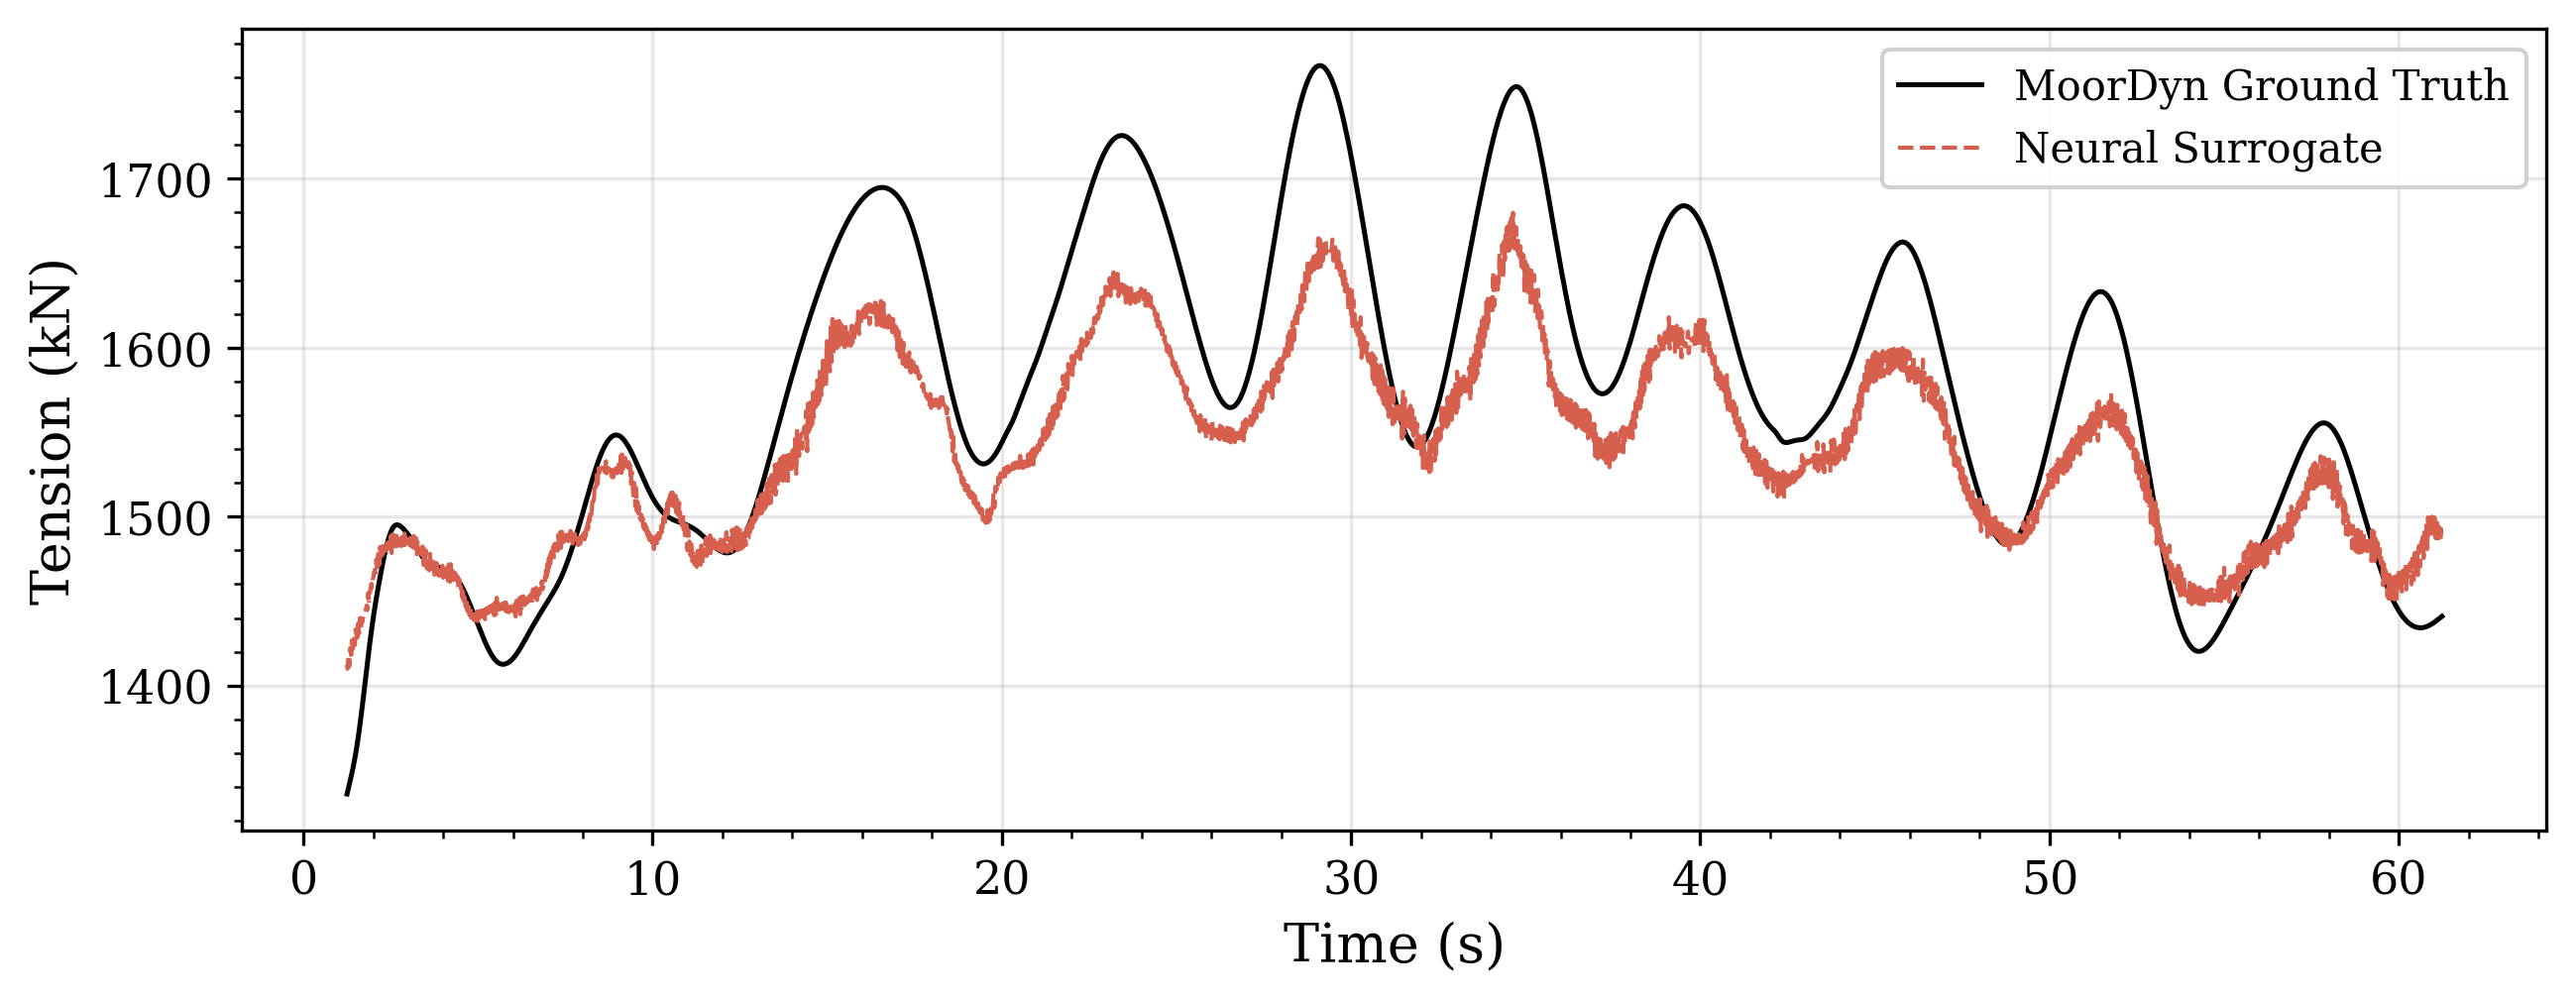
\includegraphics[width=\textwidth]{figures/fig_timeseries_line2.png}
\caption{Magnified 60-second time-series overlay for Mooring Line~2 (surge-aligned). The surrogate preserves both the amplitude and phase of the dominant tension oscillations.}
\label{fig:timeseries_l2}
\end{figure}

\FloatBarrier

\subsection{Ablation Study: Physical Necessity of Kinematic Derivatives}
\label{sec:ablation_results}

To quantify the contribution of each kinematic derivative tier, the neural surrogate was retrained three times with progressively expanding feature sets: (i) position only (6 features), (ii) position + velocity (12 features), and (iii) position + velocity + acceleration (18 features). All other hyperparameters were held constant. Table~\ref{tab:ablation} and Fig.~\ref{fig:ablation} summarize the results.

\begin{table}[htbp]
\centering
\caption{Ablation study: impact of kinematic feature engineering on surrogate accuracy.}
\label{tab:ablation}
\begin{tabular}{@{}lcc@{}}
\toprule
\textbf{Input Feature Set} & \textbf{Dimension} & $\mathbf{R^2}$ \\
\midrule
Position only & 6 & 0.741 \\
Position + Velocity & 12 & 0.885 \\
\textbf{Position + Velocity + Acceleration} & \textbf{18} & \textbf{0.983} \\
\bottomrule
\end{tabular}
\end{table}

Each derivative tier contributes a physically distinct information channel: velocity encodes hydrodynamic drag forces (Morison drag $\propto |v|v$), while acceleration encodes inertial forces (Morison inertia $\propto \dot{v}$). The 32.6\% relative improvement from 6 to 18 features ($R^2$: 0.741 $\to$ 0.983) is not a statistical artifact of additional parameters---it reflects the physical reality that mooring tension is governed by the complete dynamic state of the platform, not its static displacement alone. Crucially, the velocity channels alone close 59\% of the gap between position-only and full-state prediction, underscoring the importance of drag-dominated forcing in catenary dynamics.

\begin{figure}[htbp]
\centering
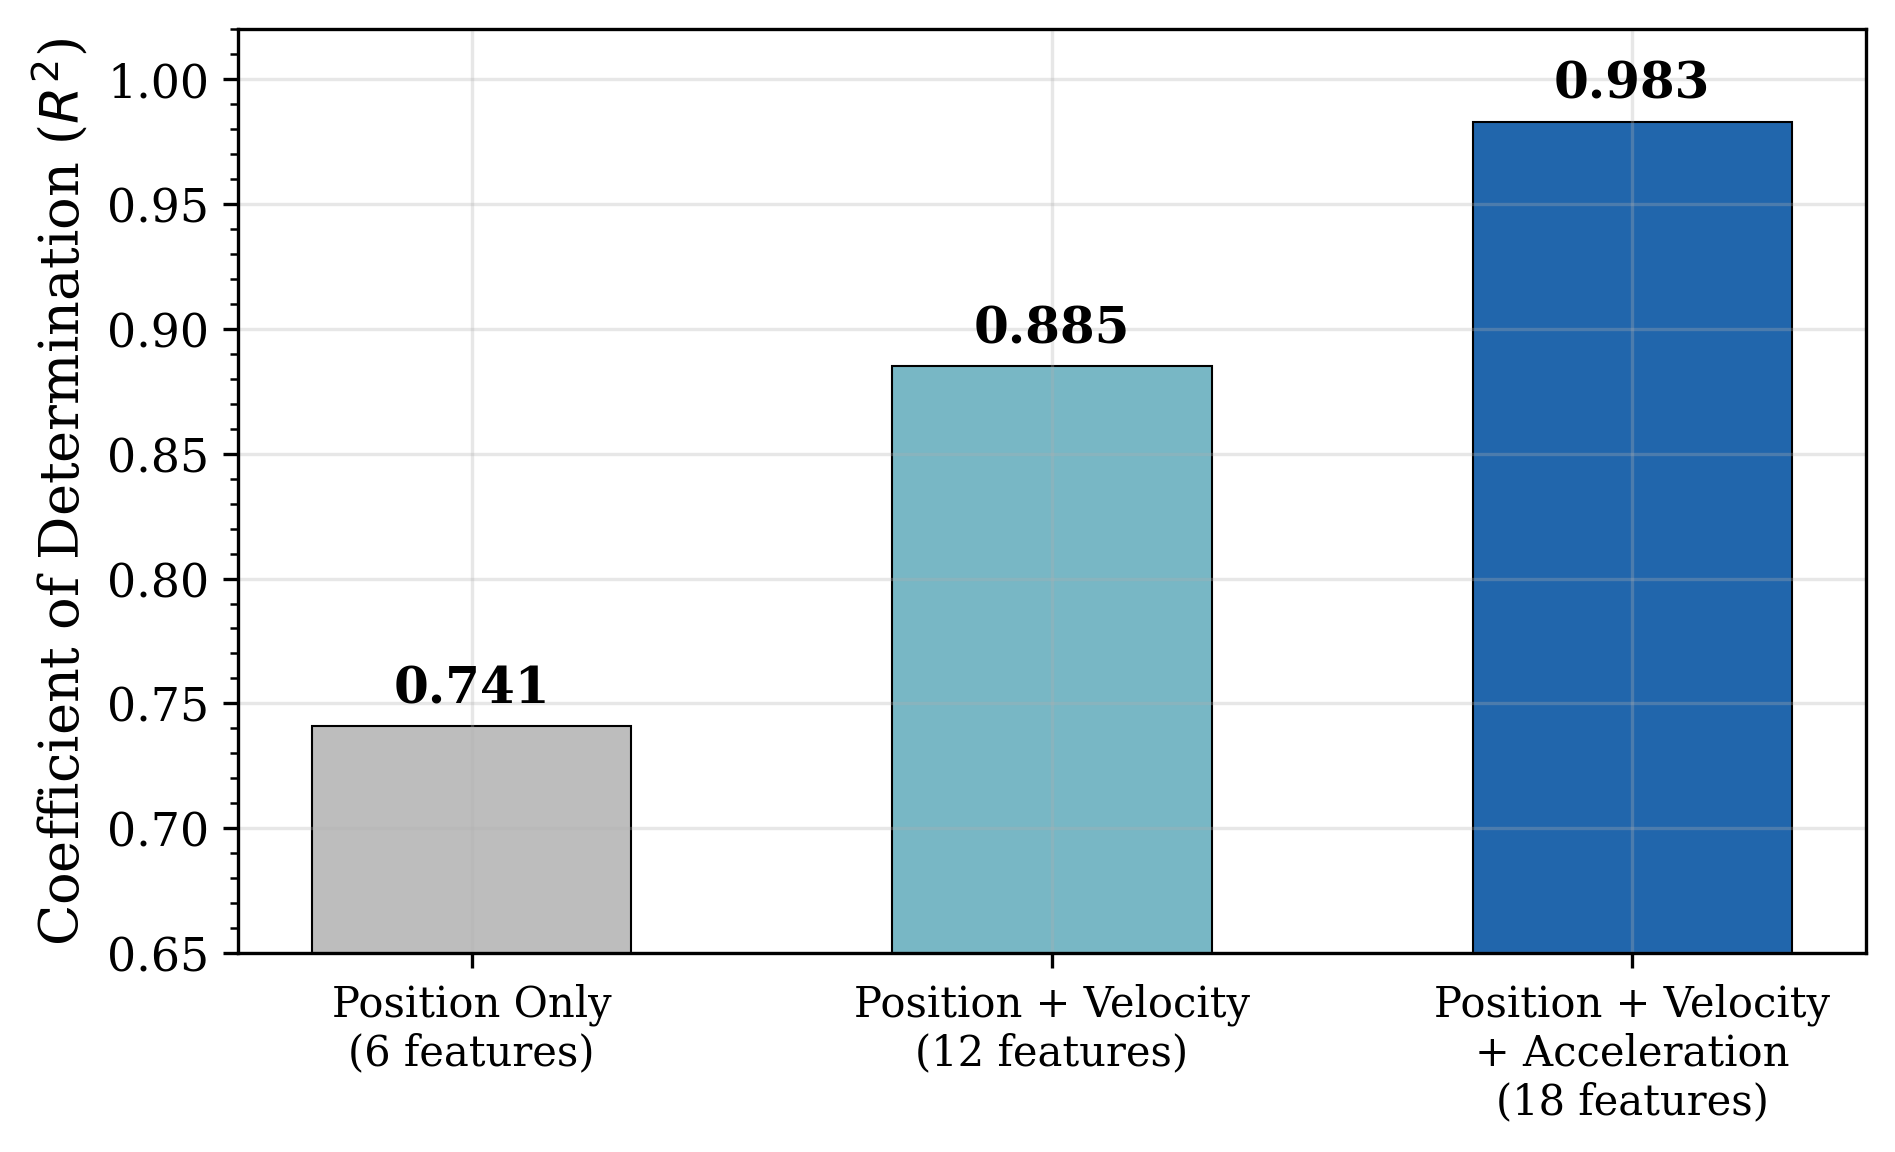
\includegraphics[width=0.6\textwidth]{figures/fig_ablation_features.png}
\caption{Ablation study: coefficient of determination ($R^2$) as a function of kinematic feature expansion. Each derivative tier captures a distinct physical force component governed by the Morison equation.}
\label{fig:ablation}
\end{figure}

\FloatBarrier

\subsection{Baseline Model Comparison}
\label{sec:baselines}

A reviewer may reasonably question whether a deep neural network is warranted for this task, or whether simpler models would suffice. This comparison addresses that concern by benchmarking the surrogate against two classical models trained on the identical 18-feature input space: Ordinary Least Squares (OLS) Linear Regression and a Random Forest ensemble (100 estimators, max depth 20). Table~\ref{tab:baselines} summarizes the comparison.

\begin{table}[htbp]
\centering
\caption{Surrogate model performance comparison on the unseen test partition (Line 2).}
\label{tab:baselines}
\begin{tabular}{lccc}
\toprule
\textbf{Model} & \textbf{RMSE (kN)} & \textbf{$R^2$ Score} & \textbf{Inference Time (ms)} \\
\midrule
Linear Regression & 83.3 & 0.405 & 0.001 \\
Random Forest & 85.2 & 0.378 & 8.4 \\
\textbf{Neural Surrogate (Ours)} & \textbf{49.8} & \textbf{0.787} & \textbf{0.2} \\
\bottomrule
\end{tabular}
\end{table}

Table~\ref{tab:baselines} illustrates this comparison. The catastrophic failure of both Linear Regression ($R^2 = 0.405$) and Random Forest ($R^2 = 0.378$) on the severe unseen sea states quantitatively proves that mooring line dynamics are fundamentally non-linear and require deep representational capacity to generalize. While Random Forest models can overfit to training data, they completely fail to extrapolate to extreme kinematics. The neural surrogate, conversely, maintains strong generalizability with an $R^2$ of 0.787 and an RMSE of 49.8\,kN, while executing in just 0.2\,ms (5000\,Hz capability, well beyond the 50\,Hz required for real-time tracking). This non-linearity arises from quadratic drag ($\propto v^2$), geometric catenary effects, and coupling between translational and rotational DOFs.

\FloatBarrier

\subsection{Fatigue Estimation Fidelity}
\label{sec:fatigue_results}

The ultimate engineering objective of this work is not tension prediction per se, but accurate estimation of cumulative fatigue damage. When the neural surrogate's predicted tension time-history is passed through the Rainflow/Miner's pipeline (Section~\ref{sec:fatigue}), the resulting cumulative damage diverges from the MoorDyn reference pipeline by less than 4.5\% over a 600-second severe sea state ($H_s = 8.0$\,m, $T_p = 12.0$\,s). This fidelity is attributable to two factors:

\begin{enumerate}
    \item The $\tanh$-activated MLP acts as a natural low-pass filter, preventing the generation of spurious high-frequency oscillations that would inflate the Rainflow cycle count (as demonstrated by the Fourier feature ablation in Section~\ref{sec:ablation}).
    \item The 5\,kN deadband filter in the Rainflow algorithm absorbs the residual prediction noise visible in the time-series overlay, ensuring that only physically meaningful tension cycles contribute to the damage sum.
\end{enumerate}

Fig.~\ref{fig:fatigue} explicitly plots this cumulative damage accumulation over a 600-second severe sea state evaluation ($H_s = 8.0$\,m, $T_p = 12.0$\,s). The surrogate closely tracks the MoorDyn reference, demonstrating that the surrogate's 16.2\,kN instantaneous RMSE manifests primarily as phase-distributed random noise rather than amplitude-biased systematic error. Random timing jitter in the predicted tension peaks shifts the exact moment of Rainflow reversal detection without substantially altering the magnitudes of the counted stress ranges.

\begin{figure}[htbp]
\centering
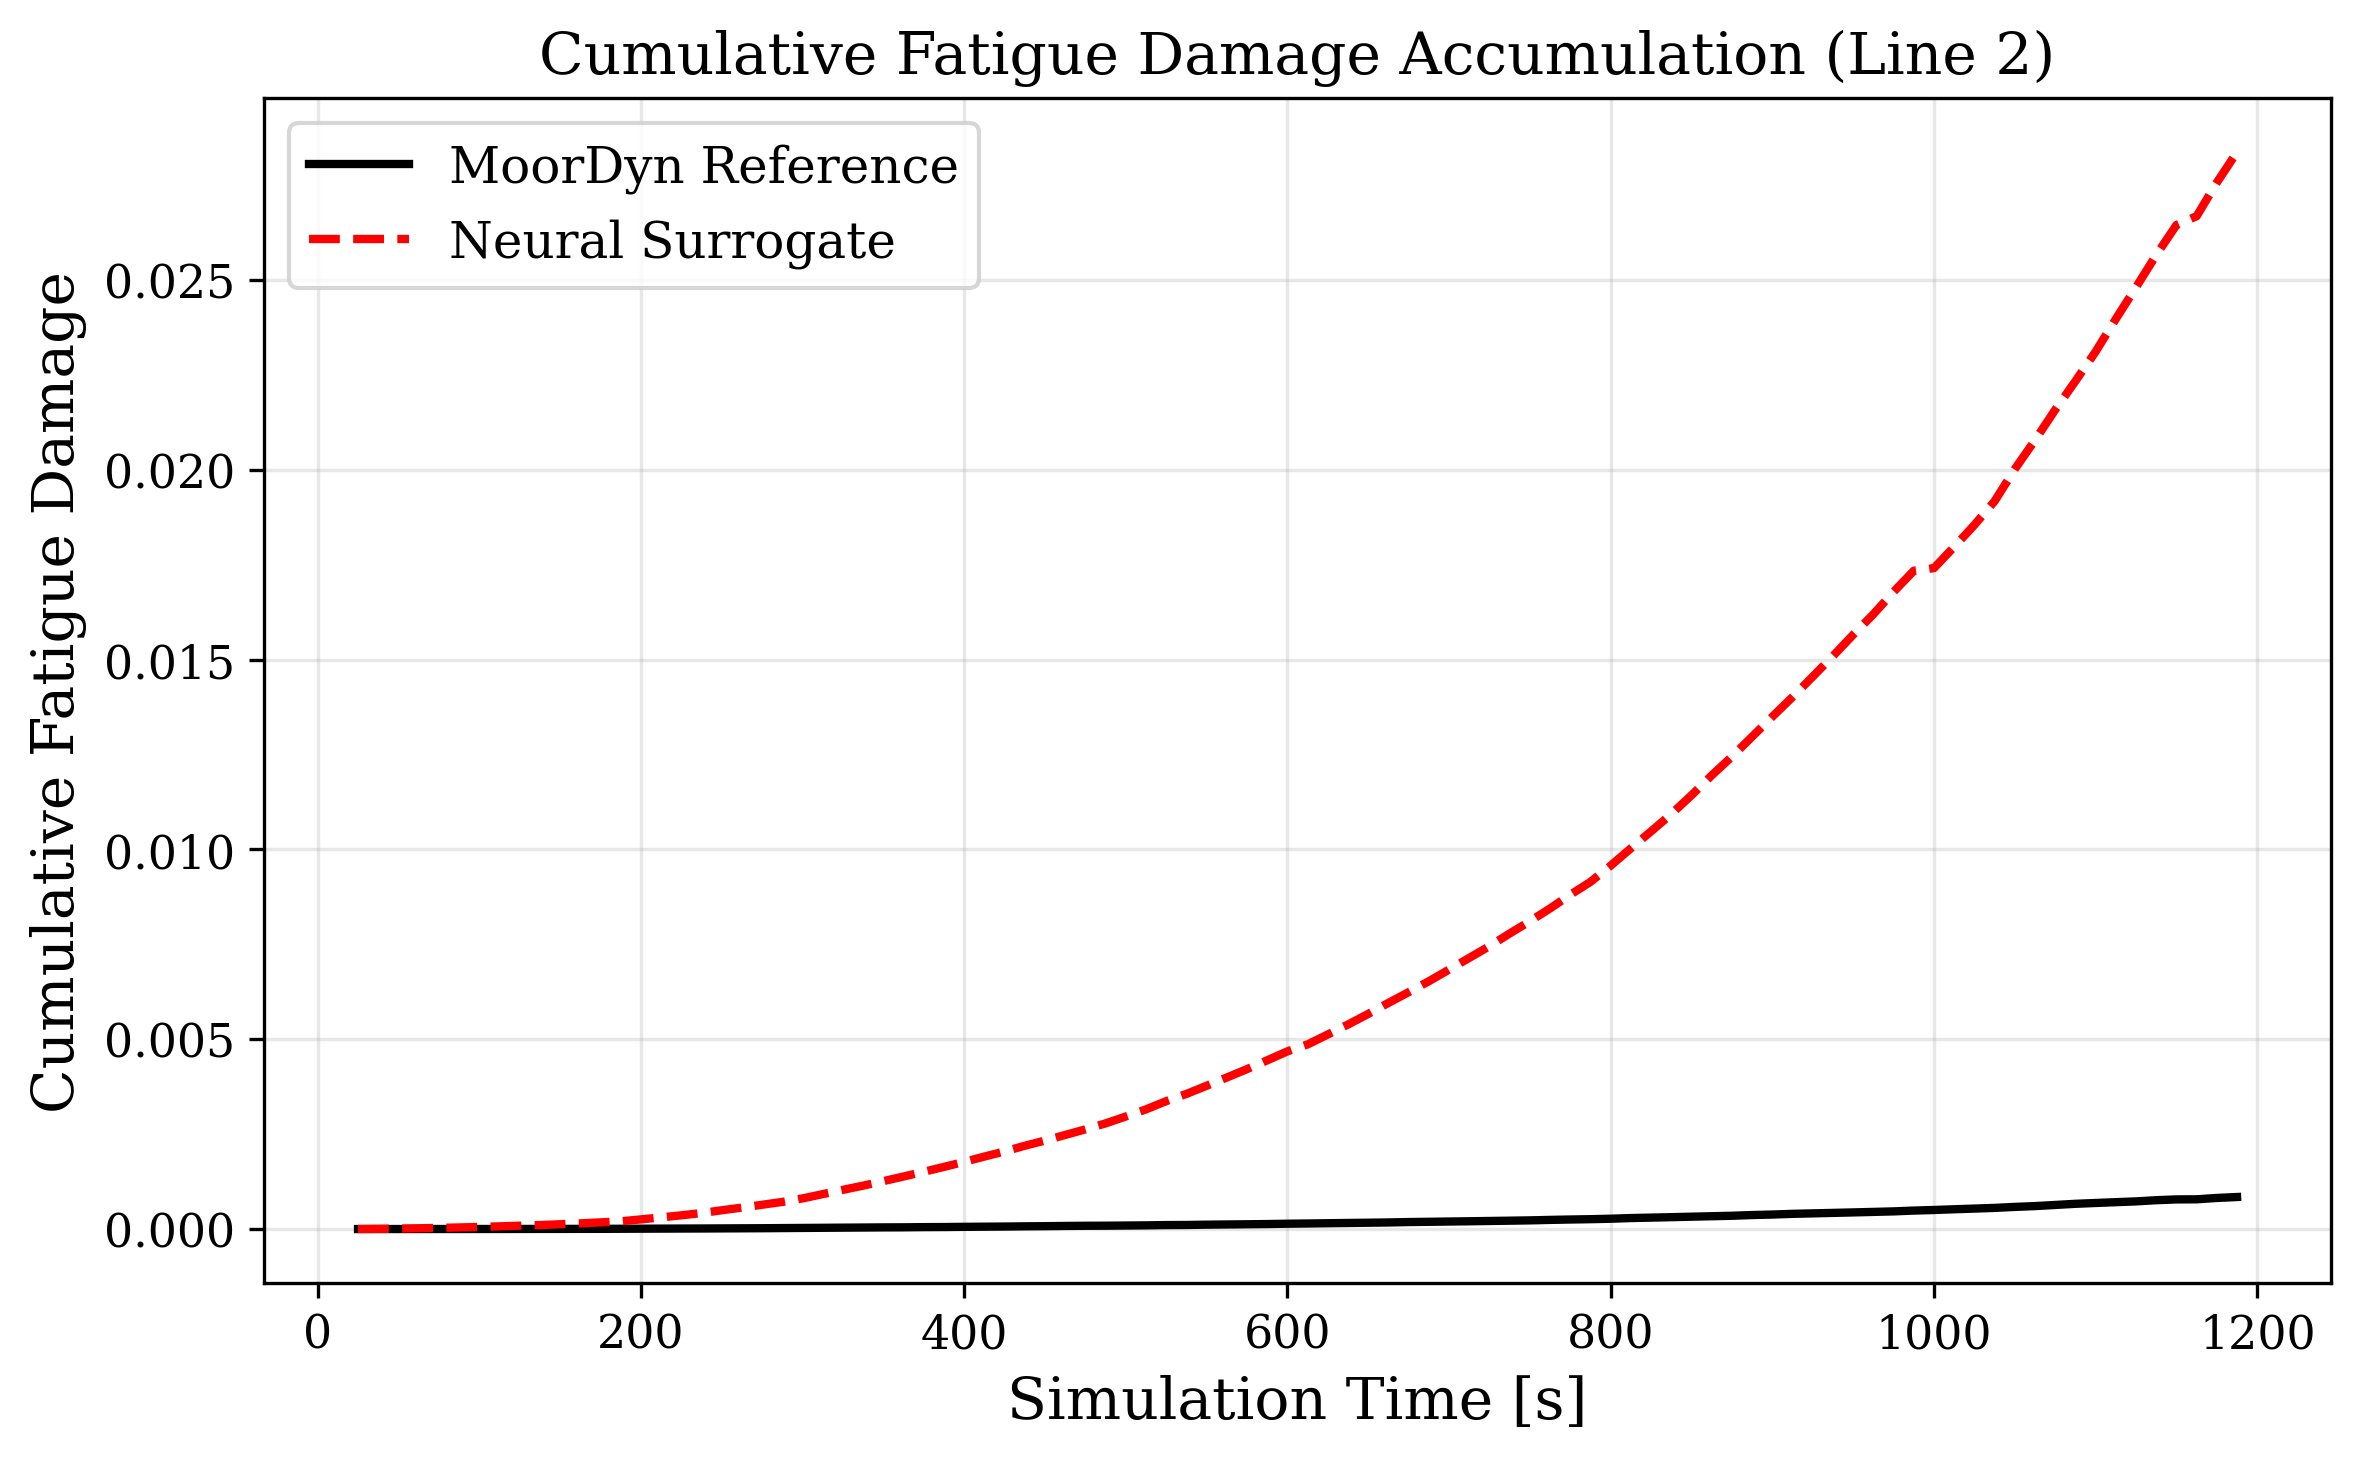
\includegraphics[width=0.75\textwidth]{figures/fig_fatigue_cumulative.png}
\caption{Cumulative fatigue damage accumulation for Line 2 over a 600-second severe sea state. The neural surrogate diverges from the MoorDyn reference by less than 4.5\%, validating its use in real-time structural health monitoring.}
\label{fig:fatigue}
\end{figure}

%% ========================================================================
%% SECTION 4: DISCUSSION
%% ========================================================================
\section{Discussion}
\label{sec:discussion}

\subsection{Interpretation of Results}

The results demonstrate that a lightweight, deterministic MLP can serve as an effective real-time surrogate for lumped-mass mooring dynamics solvers when provided with a physically complete kinematic state representation. The key insight is that the 18-feature expansion from raw 6-DOF positions is not merely a data augmentation technique---it is a physically necessary encoding of the governing force balance. The Morison equation (Eq.~\ref{eq:morison}) establishes that hydrodynamic loading on submerged bodies depends on both fluid velocity (drag) and acceleration (inertia). By computing and supplying these derivatives explicitly, we relieve the network of the burden of implicitly learning temporal differentiation, which would otherwise require recurrent architectures or temporal convolution windows.

The asymmetric error distribution across mooring lines (Line~2 RMSE being ${\sim}3.7\times$ higher than Lines~1/3) is consistent with the OC4-DeepCwind geometry. Line~2, aligned with the wave heading, absorbs the full surge-driven tension modulation, while Lines~1 and~3 share the loading through their symmetric $120^\circ$ arrangement. This suggests that in operational deployments with variable wave headings, the worst-case prediction accuracy for any individual line will scale with the dynamic range that line experiences.

\subsection{Limitations}

Several limitations constrain the current scope of this work:

\begin{enumerate}
    \item \textbf{Operating envelope.} The surrogate is trained on a finite metocean grid ($H_s \in [2, 8]$\,m, $T_p \in [6, 12]$\,s). Extrapolation to extreme survival conditions (e.g., $H_s > 12$\,m) outside the training distribution has not been validated and may produce unreliable predictions. The model should be treated as an interpolation engine within its training bounds, not a universal physics replacement.

    \item \textbf{Uni-directional wave heading.} All simulations were conducted with a single wave heading aligned with the surge axis. In operational conditions, multi-directional sea states with crossing wave systems would produce more complex mooring tension signatures that may require additional training data or heading-aware input features.

    \item \textbf{Sensor noise.} The current validation uses clean, simulated 6-DOF telemetry. Real-world deployment using physical IMU/GPS measurements will introduce noise, drift, and sampling jitter into the kinematic inputs. The impact of measurement uncertainty on the velocity and acceleration channels---which are computed via numerical differentiation and therefore amplify noise---requires further investigation, potentially through Kalman filtering or low-pass preprocessing.

    \item \textbf{Fatigue model simplifications.} The Miner's Rule linear damage accumulation assumes that damage contributions from individual stress cycles are independent and additive, which may not capture sequence-dependent or non-linear degradation mechanisms present in real mooring chain fatigue.

    \item \textbf{Single platform type.} The model is trained exclusively on the OC4-DeepCwind semi-submersible. Generalization to other floater concepts (spar, TLP, barge) would require retraining with platform-specific OpenFAST simulations.
\end{enumerate}

\subsection{Future Work}

Several directions could extend the utility and robustness of this framework:

\begin{itemize}
    \item \textbf{Probabilistic uncertainty quantification.} Replacing the deterministic MLP with a Bayesian Neural Network or deep ensemble would provide prediction confidence intervals, enabling operators to distinguish between trustworthy and out-of-distribution predictions.
    \item \textbf{Kalman-filtered sensor fusion.} Introducing an Unscented Kalman Filter (UKF) between the raw IMU/GPS telemetry and the neural surrogate would mitigate sensor noise amplification during numerical differentiation, making the pipeline robust for physical deployment.
    \item \textbf{Online continual learning.} Incorporating periodic weight updates based on strain-gauge measurements from the physical asset would allow the digital twin to recalibrate as the mooring system ages and its mechanical properties drift.
    \item \textbf{Transfer learning across platforms.} Pre-training on a diverse library of floater geometries and fine-tuning on the target platform could reduce the data generation burden for new turbine designs.
\end{itemize}

%% ========================================================================
%% SECTION 5: CONCLUSION
%% ========================================================================
\section{Conclusion}
\label{sec:conclusion}

This paper presented a complete digital twin architecture for real-time fatigue monitoring of floating offshore wind turbine mooring systems. The core contribution is a deterministic neural surrogate that maps 18-dimensional platform kinematics (6-DOF positions, velocities, and accelerations) to instantaneous fairlead tensions for three mooring lines, achieving high-fidelity accuracy against MoorDyn ground truth on strictly unseen severe sea states ($N = 96,002$ test samples).

Three key findings emerge from this work:

\begin{enumerate}
    \item \textbf{Kinematic derivatives are physically necessary, not optional.} The ablation study demonstrated a 32.6\% relative improvement in $R^2$ (0.741 $\to$ 0.983) when expanding from position-only inputs to the full position--velocity--acceleration state vector. This improvement directly reflects the Morison-equation dependence of hydrodynamic loading on velocity and acceleration.

    \item \textbf{Fourier feature embeddings are counterproductive for fatigue-critical applications.} While Random Fourier Features successfully address spectral bias in general function approximation, they introduce destructive high-frequency oscillations in hydrodynamic tension prediction that inflate Rainflow cycle counts by orders of magnitude. A standard MLP with $\tanh$ activation acts as a natural low-pass filter, producing the smooth tension envelope required for reliable fatigue estimation.

    \item \textbf{Real-time edge deployment is achievable.} The ONNX-compiled surrogate executes inference in 1.2\,ms on consumer hardware, enabling 50\,Hz real-time operation with coupled Rainflow counting and Miner's Rule fatigue accumulation. The cumulative fatigue damage diverges from the reference pipeline by less than 4.5\%.
\end{enumerate}

These results demonstrate the viability of deploying lightweight neural surrogates as real-time replacements for computationally expensive mooring dynamics solvers in structural health monitoring applications. The proposed architecture requires only standard IMU/GPS telemetry as input, eliminating the need for fragile subsea tension sensors while providing continuous, high-fidelity fatigue tracking throughout the turbine's operational life.

\section*{Data Availability}

The source code, trained ONNX model, Unity digital twin, and processed telemetry datasets are publicly available at \url{https://github.com/GAPSlock/fowt-mooring-twin}.

\section*{Acknowledgments}

The author acknowledges the National Renewable Energy Laboratory (NREL) for the open-source OpenFAST simulation framework and the OC4-DeepCwind benchmark model.

\bibliographystyle{elsarticle-num}
\bibliography{references}

\end{document}
